%1234567890123456789012345678901234567890123456789012345678901234567890123456789
\chapter{Background}

\revised{The aim of this chapter is to review relevant prior work done in
  computer graphics and robotics, and biomechanics. 
  We will start with a brief discussion on various physics-based animation
  techniques for generating realistic and agile motions of virtual humanoids. 
  We then briefly outline control strategies for reducing damage of humanoid
  falls in both robotics and graphics, which inspired the proposed falling 
  strategies in this dissertation. 
  Afterward, we will review the \emph{human-in-the-loop} principle, which is
  adopted for designing our learning framework for general agile motions. 
  Because this dissertation proposes several policy search algorithms for
  optimizing the controllers in simulation and deploying them on hardware, we
  will conclude this chapter with a review of relevant prior optimization
  techniques in computer graphics and robotics. }

%% In \secref{related_dynamic}, I will start with a brief introduction on
%% popular animation techniques to generate highly dynamic motions
%% of biped characters in the physics-based simulation.
%% In \secref{related_falling}, I will review previous methods for controlling
%% falling motions of humanoids to reduce damage to body parts.
%% In \secref{related_hitl}, I will briefly summarize prior interactive
%% interfaces for selecting parameters, especially under the 
%% \emph{human-in-the-loop optimization} paradigm, which is
%% adopted in this dissertation for incorporating interactive user interventions
%% in a controller design process.
%% In \secref{related_policy}, I will review various policy search techniques and
%% optimization algorithms in both computer graphics and robotics that find
%% optimal control parameters for humanoids.

\section{Physics-based simulation of agile motor skills}
\label{sec:related_dynamic}

\revised{Throughout the entire sessions, this dissertation utilizes physics
  simulation to generate agile motions of virtual characters and test control
  policies before deploying on real robots.
  Various physics-based animation techniques have been proposed in computer
  graphics to plan and control various motor skils, ranging from locomotion to
  agile stunts of Parkour. }

\subsection{Physics-based simulation for character animation}
Physics-based character animation is a promising approach to creating
realistic and interactive animations, but designing controllers
remains difficult largely due to the complex relationship between the
control and the state variables. 
Early work \cite{Hodgins:1995:AHA,Wooten:1998:Phd} demonstrated that 
a variety of motions can be achieved by controlling the individual joints with
manually designed state machines. Since this seminal work was
published, researchers in computer animation have been searching for
new control algorithms that are more robust, more generalizable, and
more automatic. 
Using motion capture data for reference
trajectories was a step toward a more automatic process for controller
design 
\cite{Zordan:2005:DRM,Sok:2007:SBB}, 
however, the simulated motions
cannot deviate much from the input data. An improved approach applied
linear or nonlinear quadratic regulators to track reference
trajectories, leading to more robust controllers against perturbations
\cite{daSilva:2008:ISS,Muico:2009:CNC}. Combination of PD servos and a
specialized balance controller driven by a simple state machine was a
very successful strategy \cite{Yin:2007:SIM}, which enabled much
follow-on work in biped control 
\cite{Wang:2009:OWC,Coros:2010:GBW,Lee:2010:DDB,Jain:2011:CPC}. 
Global planning of momentum
has also been applied to a wide range of motion from standing balance
\cite{Macchietto:2009:MCB} to locomotion 
\cite{Mordatch:2010:RPL,Ye:2010:OFC}
to highly dynamic motion 
\cite{Ha:2012:FAL,Liu:2012:TRC,AlBorno:2013:TOF,Zordan:2014:CRD}
Coros \etal adopted Jacobian transpose control from robotics literature
\cite{Sunada:1994:ACJ} to generate stable biped and quadruped
locomotion \cite{Coros:2010:GBW,Coros:2011:LSS}. Ha \etal further
demonstrated the effectiveness of the Jacobian transpose control on
dynamic stunts 
\cite{Liu:2010:SCM,Ha:2012:FAL,Ha:2014:ITD}.

\subsection{Physics-based controllers for agile motions}
\revised{Physics-based controllers for agile motions are more extensively
  developed in virtual simulation due to the limitation of hardware.
  The work presented in Chapter 3, 5, and 6 was inspired by prior
  animation techniques designed for various motor tasks.}
Previous work has demonstrated that highly
dynamic motions with a long ballistic phase can be synthesized using
physics simulation or kinematic approaches. Hodgins \etal
\cite{Hodgins:1995:AHA,Wooten:1998:Phd} showed that carefully
crafted control algorithms can simulate highly athletic motions,
including diving, tumbling, vaulting, and leaping. Faloutsos \etal
\cite{Faloutsos:2001:CCF} composed primitive controllers to
simulate more complex motor skills, such as a kip-up move or a dive
down stairs. Liu \etal \cite{Liu:2010:SCM} successfully tracked
contact-rich mocap sequences using a sampling-based approach. They
showed that vigorous motions with complex contacts, such as a
dive-roll or a kip-up move, can be dynamically simulated, provided
full body mocap sequences as desired trajectories. Zhao and van de
Panne \cite{Zhao:2005:UII} provided a palette of parametrized
actions to build a user interface for controlling highly dynamic
animation.  Other techniques directly edit ballistic motion sequences
under the constraints imposed by conservation of momentum
\cite{Majkowska:2007:FPM,Sok:2010:EDH}, or apply a hybrid method for
synthesizing dynamic response to perturbation in the environment
\cite{Shapiro:2003:HCI}.  If the contact positions and timing are
known, spacetime optimization techniques can also generate compelling
dynamic motions
\cite{Liu:2002:SCD,Fang:2003:ESP,Safonova:2004:SPR,Sulejmanpavic:2004:APB}.
This thesis the approach of physical simulation, 
but we seek for a more general and robust control algorithm such that the
controller can operate under a wide range of initial conditions and
allow for runtime perturbations. 



\section{Control of humanoid falls}
\label{sec:related_falling}
\revised{A goal of falling strategies is to minimize damage or joint stress to
  humanoid when it falls.
  This is an important problem to protect virtual and real humanoids during
  learning and executing agile motor skills, which has
  been well studied within a variety of research areas, such as computer
  graphics, robotics, biomechanics, and martial arts}

\subsection{Falling detection techniques}
\revised{Although the falling strategies proposed in Chapter 3 and 4 majorly
  focus on reducing damage to body parts, they require a fall detection module
  for predicting and estimating falls, which is assumed in this disseration.
  It will predict a fall and try to recover the balance if it is possible,
  and activate a falling controller if it is needed.}
%% To activate a falling controller, a robot first predicts a fall and
%% try to recover the balance if it is possible.
Various machine learning techniques has been proposed to detect falls, such as
Principal Component Analysis \cite{Karssen:2008:FDW} or 
Supported Vector Machine \cite{Kim:2011:MLA}.
Horn and Gerth \cite{Hohn:2009:PBM} detects unstable situations with
Gaussian Mixture Model or Hidden Markov Model
and activates appropriate reflex controls, such as crouching. 
Renner and Benke \cite{Renner:2006:IDF} proposed to detect instability using
an aggregated sensor deviation and stabilize the gait with manually designed
reflex controllers. 
The falling strategies presented in this dissertation focus
on control of falling motions to reduce damage when the
robot detects falling, presumably with one of the above techniques. 

\subsection{Falling damage reduction strategies}
\revised{In this section, we will review the related work on the falling
  strategies proposed in Chapter 3 and 4.
  Various techniques in different disciplines have been proposed to minimize
  damage on humanoid when falling is inevitable. }
%% When a robot is pushed hard and falling is inevitable, 
%% various techniques has been proposed to minimize damage on humanoid. 
Fujiwara \etal
\cite{Fujiwara:2002:UFM,Fujiwara:2003:FHH,Fujiwara:2006:TOF,Fujiwara:2007:OPF}
proposed falling techniques inspired by Japanese martial arts (\emph{Ukemi}).
Ogata \etal \cite{Ogata:2007:FMC,Ogata:2008:RSG} evaluates the risk of falling with
predicted ZMP and optimizes COM trajectories to reduce damage. 
Ruiz-del-Solar \etal \cite{Ruiz:2009:LTF,Ruiz:2010:FDM} designed low damage
falling sequences for soccer robots and verified them in the simulation. 
Wang \etal \cite{Wang:2012:WTO} formulated an optimization of whole body
trajectories as a nonlinear programming problem and solved it with heuristics.
Lee and Goswami \cite{Lee:2012:FOB} proposed a control strategy that
reorients the robot to fall with a backpack for absorbing shock. 
Yun and Goswami \cite{Yun:2014:TFC} addressed a ``tripod'' strategy that
stops with a swing foot and two hands to maintain the final COM location
higher from the floor.   
To protect the surrounding environment, \cite{Goswami:2014:DCF} proposed a
fall direction-changing strategy that utilizes foot placement and inertia
shaping.
% However, most of falling strategies assume the specific sequence of contacts
% that is specialized to the given scenarios, such as ``hands''
% \cite{Ogata:2007:FMC}, ``knee-and-hands'' \cite{Fujiwara:2007:OPF}, or
% ``foot-and-hands'' \cite{Yun:2014:TFC}. 

\revised{Besides the related work for falls caused by external perturbations,
  there are additional works that focus on falls from higher
  places.}
In those cases, control strategies during long airborne phase
become critical for safe landing.
\revised{The falling algorithm in Chapter 3 draws} inspiration from
kinesiology literature and sport practitioners. In particular, the
techniques developed in freerunning and parkour community are of
paramount importance for designing landing control algorithms capable
of handling arbitrary scenarios
\cite{Edwardes:2009:TPF,HLJ:2011:URL}. 
In robotics, Bingham \etal \cite{Bingham:2014:OMA} proposed an algorithm 
that leverages nonholonomic trajectory planning inspired by the
falling cat to orient an articulated robot through configuration
changes to achieve a pose that reduces the impact at landing.

%% \subsection{Falling strategies of animals}
\begin{figure}[htbp]
\center
  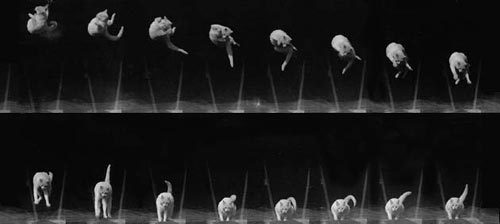
\includegraphics[width=\linewidth]{images/related_cat.jpg}
  \caption{A cat is able to right itself as it falls to land on 
  its feet, irrespective of its initial orientation.}
 \label{fig:related_cat}
\end{figure}

Many animals have astonishing capabilities to achieve different
maneuvers in the air by manipulating their body articulations.  Cats
are known for landing with feet from any initial falling condition
\cite{Kane:1969:DEF,Montgomery:1993:GTF,Cat:2015:URL}
(\figref{related_cat}). Lizards swing their tails to
stabilize their bodies during a leap \cite{Libby:2012:TAP}. Pigeons
reorient their bodies to achieve a sharp turn when flying at low speed
\cite{Ros:2011:PSL}. These behaviors inspire scientists and engineers
to develop intelligent devices and control algorithms. This dissertation has a
similar goal that we study how human body can change shape in the
air to reduce damage at landing.

%% \section{Interactive interfaces}

%% \subsection{Parameter selection interfaces}
%% \karen{What is the context of this section?}
%% \karen{Doesn't sound relevant your thesis}
%% A common approach in parameter selection interfaces is 
%% to present the parameter space (or a collection of samples thereof) in an explorable way,
%% through 2D layout of results \cite{Marks:1997:DGA};
%% careful selection of sliders \cite{Ovsjanikov:2011:Shapes,Lindow:2012:PLP};
%% or (in a physics context) direct manipulation \cite{Popovic:2000:IMR}
%% %Possibly cite mesh keyframing here as well
%% or in-situ visualization \cite{Twigg:2007:MWB}.
%% Both \cite{WFR:2010:WL,WFR:2011:NOR} represent simulations as tracks (or word lines) 
%% where each parameter change corresponds to branches that spawn new tracks, and 
%% \cite{WFR:2010:WL} describes how to incorporate uncertain parameter values into this explorable visualization.  
%% Meanwhile \cite{BM:2010:RDE} clusters outcomes from different timelines to suppress minor variations and to highlight entire outcome categories. 
%% These methods help a designer understand the effects of parameter variation 
%% on a single set of initial conditions.

\section{Human-in-the-loop interfaces}
\label{sec:related_hitl}
%% Without human guidance, fully automated optimization algorithms
%% sometimes produce undesired solutions due to unexpected factors or
%% situations \revised{which are not considered in the objective function or
%%   constraints.}

Without human guidance, fully automated optimization algorithms
sometimes produce undesired solutions due to unexpected factors or
situations.
\revised{For instance, finding the optimal jumping motion with the desired
  height can be achieved in many different joint trajectories.
  Although many trajectories can achieve lower objective values, excessive
  usages of hips or heels make jumping motions abnormal.
  In Chapter 5, we propose the semi-automatic learning framework which involves
  a human in the optimization process to effiently find optimal and natural
  motions within a short amount of time.}
%% To fill the gap, researchers have developed
%% semi-automatic systems which involve a human in the process to provide
%% prior knowledge and guidance to the
%% optimization.
%% \cite{Scott:2002:IHC}. 
\revised{This paradigm is so called \emph{human-in-the-loop} (HITL) 
optimization, which has} proven effective for various problems, such as
%% space shuttle scheduling \cite{Chien:1999:APS}, 
vehicle planning \cite{Waters:1984:IVR} or interface optimization
\cite{Quiroz:2007:IEX}.  The level of user interaction
varies from simply selecting of the generated solutions
\cite{Sims:1991:AEC} to directly editing the search parameters and
constraints \cite{Sreevalsan-Nair:2007:HGE}. Unlike
most previous work which primarily focused on developing user
interaction and visualization techniques for HTIL optimization
systems, we develop a new controller design framework that exploit the nature of
HITL computation paradigm.

\section{Policy search algorithms}
\label{sec:related_policy}
\revised{In Chapter 6, 7, and 8, we describe policy search algorithms for
  finding optimal controllers.
  In this section, we will review existing algorithms that are classified into
  two categories based on the existance of simulation models.
  We will also cover related work on special cases, optimization of
  parameterized motor skills.}

\subsection{Model-free policy search algorithms}
\revised{Chapter 6 and 7 are inspired by existing model-free policy
  optimization techniques where the policy is improved through a number of
  hardware trials~\cite{bib-morimoto-standup,bib-kober-primitives}. }
%% In robotics, a common techniques for searching optimal policy parameters is 
%% model-free policy optimization, 
%% where the policy is improved through a number of hardware 
%% trials~\cite{bib-morimoto-standup,bib-kober-primitives}.
Unfortunately, these methods generally require hundreds of
trials, which is unrealistic for tasks such as humanoid balancing and
locomotion.
One way to overcome this issue is to limit the parameter space by using
task-specific primitives~\cite{bib-nakanishi-adaptation} or to provide a
good initial trajectory by human
demonstration~\cite{bib-atkeson-demonstration}.
However, it is not clear how to extend these approaches to dynamically
unstable robots or tasks that cannot described by joint trajectories.

Various optimization techniques have been applied to improve the
motion quality or the robustness of the controller.  In character
animation, a sampling-based method, Covariance Matrix Adaption
Evolution Strategy (CMA-ES) \cite{Hansen:2004:CMA}, has been
frequently applied to discontinuous control problems, such as biped
locomotion \cite{Wang:2009:OWC,Wang:2010:OWC,Wang:2012:OLC},
parkour-style stunts\cite{Liu:2012:TRC,Ha:2014:ITD}, or swimming
\cite{Tan:2011:ASC}.  To compensate the expensive cost of
sampling-based algorithm, different approaches have been proposed,
including exploiting the domain knowledge
\cite{Wang:2009:OWC,Wang:2010:OWC,Wang:2012:OLC}, shortening the
problem horizons \cite{Sok:2007:SBB}, or using a classifier to exclude
infeasible samples \cite{Ha:2014:ITD}. Based on the previous success
of CMA-ES, we proposed new sampling-based algorithms that resemble the
evolution process of distribution.

\subsection{Model-based policy search algorithms}
\begin{figure}[htbp]
\center
  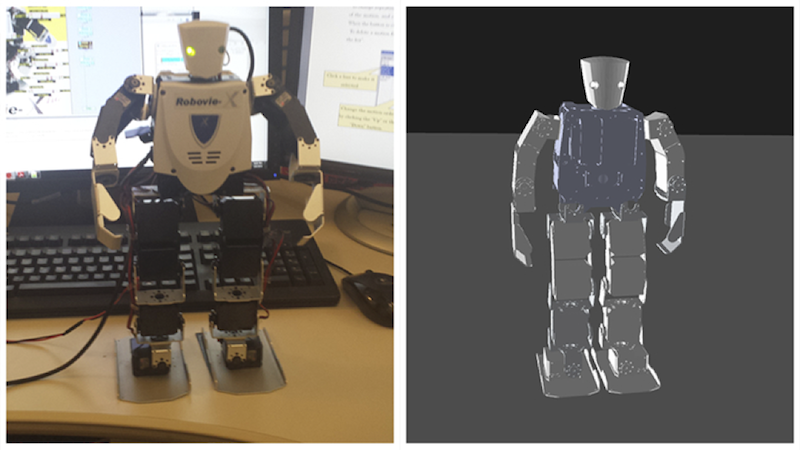
\includegraphics[width=0.9\linewidth]{images/related_robovies.png}
  \caption{Difference between a real robot and its simulation model
  results different motions from same controllers.}
 \label{fig:related_robovies}
\end{figure}

\revised{Chapter 8 proposed a model-based policy search algorithms that
  utilizes simulation to reduce the number of hardware trials.
  In this category of algorithms,}
difference between a robot and its simulation model becomes a serious 
problem  (\figref{related_robovies}).
%% when we try to use controllers obtained by model-based
%% optimization or tuned in simulation (\figref{related_robovies}).
Classical parameter identification
techniques~\cite{bib-khalil-identification} partially solve this
problem by fitting model parameters to experimental data, but they
are still limited to factors that can actually be modeled. 
Furthermore, these approaches assume that the data set is large enough
to accurately estimate the parameters.
In large and unstable systems such as humanoid robots, it is often
difficult to collect enough data~\cite{bib-humanoids2011-calibration}.

A number of researchers have attempted to overcome the drawbacks of
these approaches by combining simulation and real-world data~
\cite{bib-sutton-integrated,bib-moore-prioritized-sweeping,bib-peng-incremental}.
Abbeel et al.~\cite{bib-abbeel-inaccurate} used an inaccurate model to
estimate the derivative of the cost with respect to the policy
parameters.
Ko et al.~\cite{bib-ko-blimp} used Gaussian Process to model the
difference between a nonlinear dynamics model and the actual dynamics
and applied the model to reinforcement learning for yaw control of a
blimp.  However, they do not iterate the process to refine the model.
Deisenroth et al.~\cite{bib-deisenroth-data-efficient} also used
Gaussian Process for learning the dynamics model from scratch.
Similarly, Morimoto et al.~\cite{bib-iros07-improving} used Gaussian
Process for learning simplified dynamics of human locomotion.
Sugimoto et al.~\cite{bib-humanoid13-trajectory} used
\emph{sparse pseudo-input Gaussian Process} (SPGP) that accounts both
variances of inputs and outputs to handle sensor noises.
Instead, Tangkaratt et al.~\cite{bib-nn14-model} used 
\emph{least-squares conditional density estimation} (LSCDE) to learn 
the dynamics model without Gaussian assumption on the transitions.
Cutler et al.~\cite{bib-icra14-reinforcement} trained a policy in 
multiple fidelity simulators with discretized actions.
Ross and Bagnell~\cite{bib-ross-agnostic} theoretically proved that
their iterative system identification method converges even the system
is not in the assumed class.
Please refer to Section 6 of~\cite{bib-kober-survey} for more complete
survey on this topic.

\subsection{Policy search algorithms for parametrized tasks}
There is a large body of research work on generalization of learned
motor skills to achieve new tasks,
\revised{which is discussed in Chapter 7.}
da Silva \etal
\cite{DaSilva:2012:LPS,DaSilva:2014:LPM,DaSilva:2014:ACP} introduced a
framework to represent the policies of related tasks as a
lower-dimensional piecewise-smooth manifold. Their method also
classifies example tasks into disjoint lower-dimensional charts and
model different sub-skills separately. Much research aimed to
generalize example trajectories to new situations using dynamic
movement primitives (DMPs) to represent control policies
\cite{Ijspeert:2002:LAL}. A DMP defines a form of control policies
which consists of a feedback term and a feedforward forcing
term. Ude \etal \cite{Ude:2010:TSG} used supervised learning to train a set of
DMPs for various tasks and built a regression model to map task
parameters to the policy parameters in DMPs. 
Muelling \etal \cite{Muelling:2010:LTT}
proposed a mixture of DMPs and used a gate network to activate the
appropriate primitive for the given target parameters.
Kober \etal \cite{Kober:2010:RLA} trained a mapping between task parameters and
meta-parameters in DMPs using a cost-regularized kernel
regression. Through reinforcement learning framework, they computed a
policy which is a probability distribution over meta-parameters.
Matsubara \etal \cite{Matsubara:2011:LPD} trained a parametric DMP by shaping a
parametric-attractor landscape from multiple demonstrations.
Stulp \etal \cite{Stulp:2013:LCP} proposed to integrate the task parameters as
part of the function approximator of the DMP, resulting in more
compact model representation which allows for more flexible
regression. 
Neumann \etal \cite{Neumann:2013:IMS} modified the existing learning
algorithm (REPS) to learn a hierarchical controller that has
parameterized options.

All these methods described above depend on collecting a set of
examples. This presents a bottleneck to learning because an individual
control policy needs to be learned for each task example drawn from
the distribution of interest. da Silva \etal further proposed using
unsuccessful policies as additional training samples to accelerate the
learning process \cite{DaSilva:2014:LPM}. For dynamic motor skills
which involve intricate balance tasks, unsuccessful policies generated
during training a particular task are of no use to other tasks because
they often lead to falling motion. 
Hausknecht \etal \cite{Hausknecht:2010:LPK}
demonstrated a quadruped robot kicking a ball to various distances,
but whole-body balance was not considered in their work.  Another
challenge regarding dynamic tasks is that each task can be achieved by
a variety of policies, some of which might be overfitting the
task. Interpolating these overfitted policies can lead to unexpected
results. In this dissertation, we proposed a new algorithm that
tends to generate more coherent mapping between
task parameters and policy parameters because we simultaneously learn
the policies for the entire range of the tasks.

\rule{\textwidth}{1pt}
The next chapter will describe falling strategies for
virtual characters and real robots, which are essential for
protecting humanoids from severe damage.
